%
%このファイルはヒューマンインタフェースシンポジウム用スタイルファイル
%hissymp.cls(ver.1.0) を利用した「原稿執筆の手引き」です。
% Revised in January, 2007 by Itiro Siio
%

\documentclass{hissymp}

%ご使用の環境にあわせてください
\usepackage[dvipdfmx]{graphicx}
%\usepackage[dviout]{graphicx}
\usepackage{url}


%和文タイトル
\jtitle{複数人で使用可能な3Dアイデアノートシステムの提案}

%著者日本名
\jauthor{
猪膝 孝之\thanks{電気通信大学大学院 情報理工学研究科} 
田野 俊一\addtocounter{footnote}{-1}\footnotemark 
橋山 智訓\addtocounter{footnote}{-1}\footnotemark 
丸谷 大樹\thanks{電気通信大学大学院 情報システム学研究科}  
}

%英文タイトル
\etitle{A Proposal of A 3D Idea Note System for Multiple People}

%著者英文名
\eauthor{
Takayuki Inohiza\thanks{Graduate School of Informatics and Engineering, The University of Electro-Communications},
Shun'ichi Tano\addtocounter{footnote}{-1}\footnotemark,
Tomonori Hashiyama\addtocounter{footnote}{-1}\footnotemark and 
Taiki Maruya\thanks{Graduate School of Information Systems, The University of Electro-Communications}
}
% 名前は、はじめの一文字だけ大文字にしてください。

\begin{document}

%maketitle は abstract と keyword の後に入れてください。

\begin{abstract}
The ideas suddenly come up and we currently take notes using paper and PC. However, it is difficult to take notes in places where there is no desk or white board  when ideas come up. Also, ideas may come to mind when talking with friends. In this study, we propose a 3D idea note system for multiple people.
\end{abstract}

\begin{keyword}	
3D, note taking, sharing, multimodal
\end{keyword}

\maketitle	



%%%%%%%%%%%%%%%%%%%%%%%%%%%%%%%%%%%%%%%%%%%%%%%%%%%%%%%%%%%%%%%%%%%%%
\section{はじめに}
%%%%%%%%%%%%%%%%%%%%%%%%%%%%%%%%%%%%%%%%%%%%%%%%%%%%%%%%%%%%%%%%%%%%%
アイデアはふとしたときに思い浮かぶことがあり、私達はそれを紙に書き留めたり、PCを利用してメモを取ることがある。しかし、アイデアが思い浮かぶのは座って作業しているときだけではなく、外で歩いているときや、机やホワイトボード等がないような場面でも突然思い浮かぶことがある。また、友人と話し合いをしているときにアイデアが連鎖的に思い浮かぶこともある。

近年、HMD(Head Mounted Display)の普及により3D空間に文字を書くことが可能になった。現在、HMDに関する多くの研究は一人で特定の場所において使うことが想定されている。現状では外などの広い空間を利用し、複数人で利用することを想定した研究は少ない。そこで、本研究では浮かんだアイデアを書き留める際に、どこでも配置できるように広い空間で利用することを想定する。広い空間上にメモを残すことができ、複数人で利用できるようなシステムの提案を行う。


%%%%%%%%%%%%%%%%%%%%%%%%%%%%%%%%%%%%%%%%%%%%%%%%%%%%%%%%%%%%%%%%%%%%%
\section{関連研究}
%%%%%%%%%%%%%%%%%%%%%%%%%%%%%%%%%%%%%%%%%%%%%%%%%%%%%%%%%%%%%%%%%%%%%
これまで多くの空間上に文字を描く研究がされてきた。椎尾ら\cite{tex1,tex2}は仮想の手描きメモによるコミュニケーションをウェアラブルコンピュータにより実現する空気ペンを試作した。空気ペンはユーザが任意の空間上に手書き情報を描画することが出来る機器である。HMDを利用することによって、空気ペンを使用して描いた手書き情報を見ることができる。ペン本体には、ジャイロセンサ、加速度センサが内蔵されており、これらにより描いた情報の記録を行う。また、床上にはRFID(Radio Frequency Identification)タグをつけることによって位置情報を取得している。問題点としては、床のRFIDタグを読み取るためにRFIDリーダーをつけた下駄を装着する必要があることや、使用できる範囲がRFIDタグがついた床上のみなので場所が限定されることがあげられる。

また、高山ら\cite{tex3,tex4}は実世界のどのような時間・場所であっても、ユーザが思い浮かんだふとしたアイデアを、生起を誘発したコンテキストに対応づけて保存し、それを他のユーザと共有できるシステムを作成した。これによってユーザは状況にあった質の良い情報を得ることが可能になった。問題点としては、多くの機器を装着しなければならないので持ち運びが大変であることや、操作が複雑なので慣れるのに時間がかかることが挙げられる。

長田ら\cite{tex5}はスマートグラスを用いた仮想空間への手書き情報共有システムを提案した。ジェスチャの認識を用いて指の追跡を行い、軌跡を描くことで手書き情報を実現した。これによって仮想空間において手書き情報を共有することができるようになった。問題点としては、どの物体の動きを捉えるか判断するため、空間への描画の開始前に認識させたい物体には特定のジェスチャを行わせる手間がかかることが挙げられる。

%%%%%%%%%%%%%%%%%%%%%%%%%%%%%%%%%%%%%%%%%%%%%%%%%%%%%%%%%%%%%%%%%%%%%
\section{本研究のコンセプト}
%%%%%%%%%%%%%%%%%%%%%%%%%%%%%%%%%%%%%%%%%%%%%%%%%%%%%%%%%%%%%%%%%%%%%


%%%%%%%%%%%%%%%%%%%%%%%%%%%%%%%%%%%%%%%%%%%%%%%%%%%%%%%%%%%%%%%%%%%%%
\section{提案するシステム}
%%%%%%%%%%%%%%%%%%%%%%%%%%%%%%%%%%%%%%%%%%%%%%%%%%%%%%%%%%%%%%%%%%%%%
ユーザが思い浮かんだふとしたアイデアを広い空間上の任意の場所に残すことができ、複数人で使用できるシステムを提案する。ハードウェアは可搬性を考慮して、マイクロソフト社のHoloLens\cite{tex6}を使用する。システムの機能としては大きく分けて三つであり、以下に詳細を述べる。

\subsection{メモを入力}
実世界の任意の3D空間上に図形や文字のメモを残す。また、これらに加えて音声によるメモも残すことも実現する。
\subsubsection{3D描画によるメモ}
実世界の3D空間上に線を引くことで立体的な図形や文字を描く。具体的な手法としては、3D空間上にタップアンドホールドをした状態を維持している間は線が表示され、ホールドを解除すると表示をやめる。タップとは人差し指を立てて、真っ直ぐ下に倒す動作であり、マウスで表すとクリックのことである。ホールドとは、タップをしてから人差し指と親指をつまむような動作であり、マウスで表すとドラッグやスクロールのことである。描いたものは立体的に見ることができるようにする(図\ref{fig:3d_draw})。

\begin{figure}[h]
  \begin{center}
    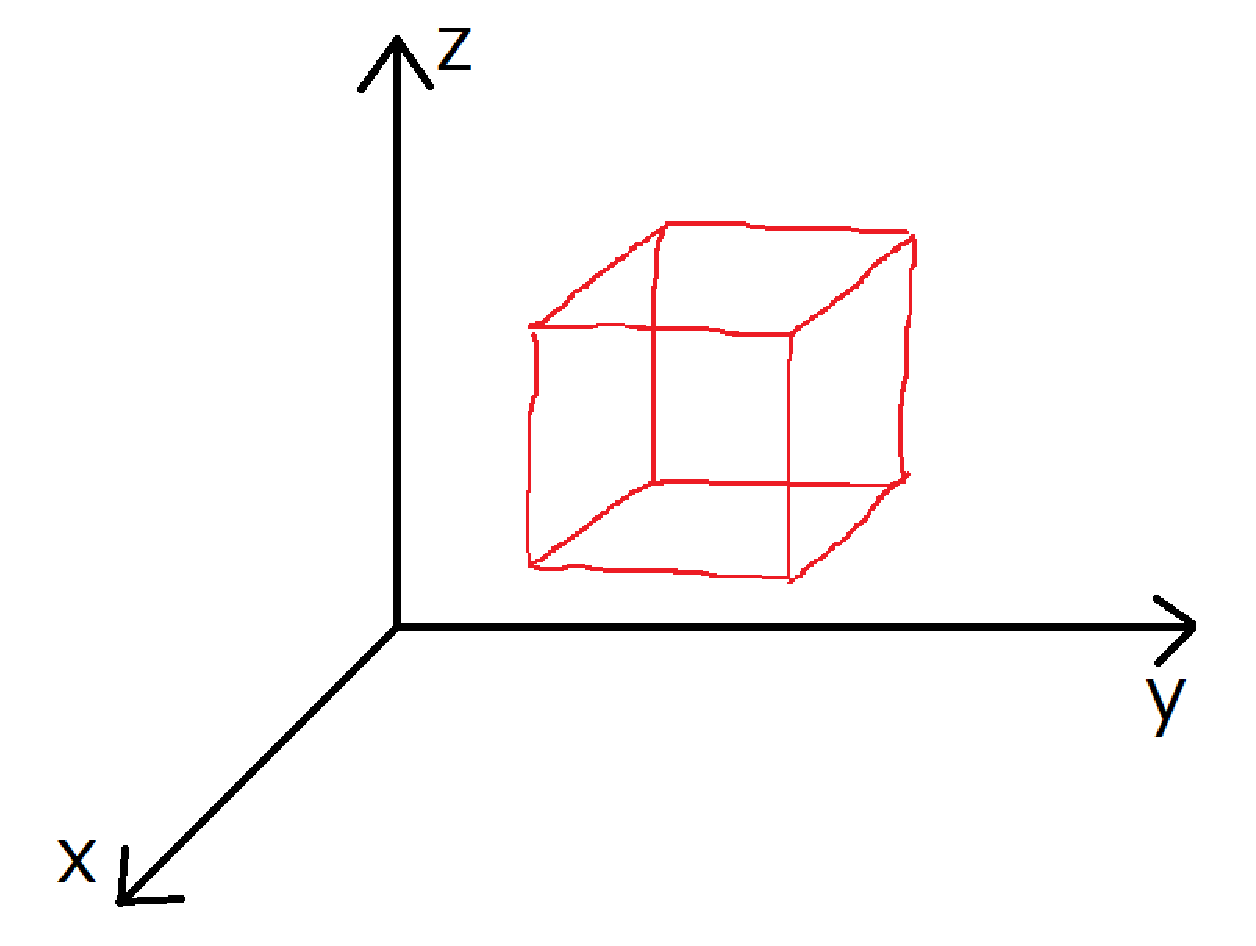
\includegraphics[clip,height=5.0cm,width=6.0cm]{./3d_draw.eps}
    \caption{3D描画によるメモ}
    \ecaption{Notes drawn in 3D.}
    \label{fig:3d_draw}
  \end{center}
\end{figure}

\subsubsection{文字描画によるメモ}
3D空間上に文字によるメモをそのまま残す場合、見る方向によっては文字として見えないと問題が発生することが考えられる。これを解決するために3D空間上に仮想平面を用意をしてその平面上に文字を描き、表示をする際に相手の方向に向けるという手法も考えられるが、リアルタイムで表示する場合、もう片方の人が文字として見えないという問題が発生することが考えられる。そこで、文字を描き、この情報を点として3D空間上に残すという手法を提案する(図\ref{fig:tennomemo})。見る際は3D空間上に残した点のメモをタップすることで文字を表示する。この手法により、どの方向から見ても文字として見ることを可能にする。

\begin{figure}[h]
  \begin{center}
    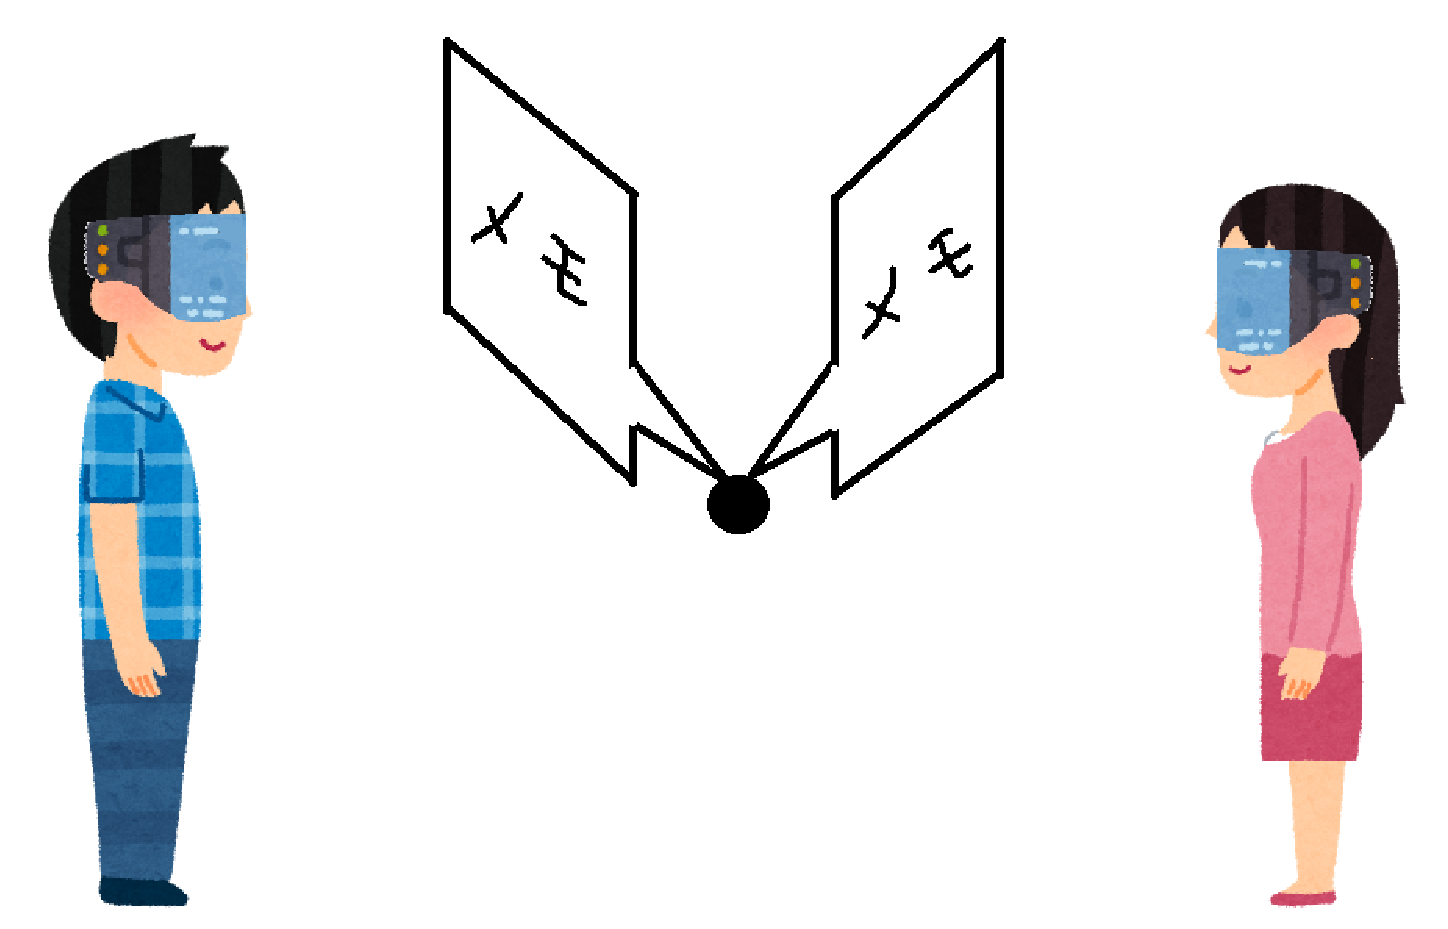
\includegraphics[clip,width=7.0cm]{./tennomemo.eps}
    \caption{点の情報としてメモを残す}
    \ecaption{Notes left as information on points.}
    \label{fig:tennomemo}
  \end{center}
\end{figure}

\begin{figure}[h]
  \begin{center}
    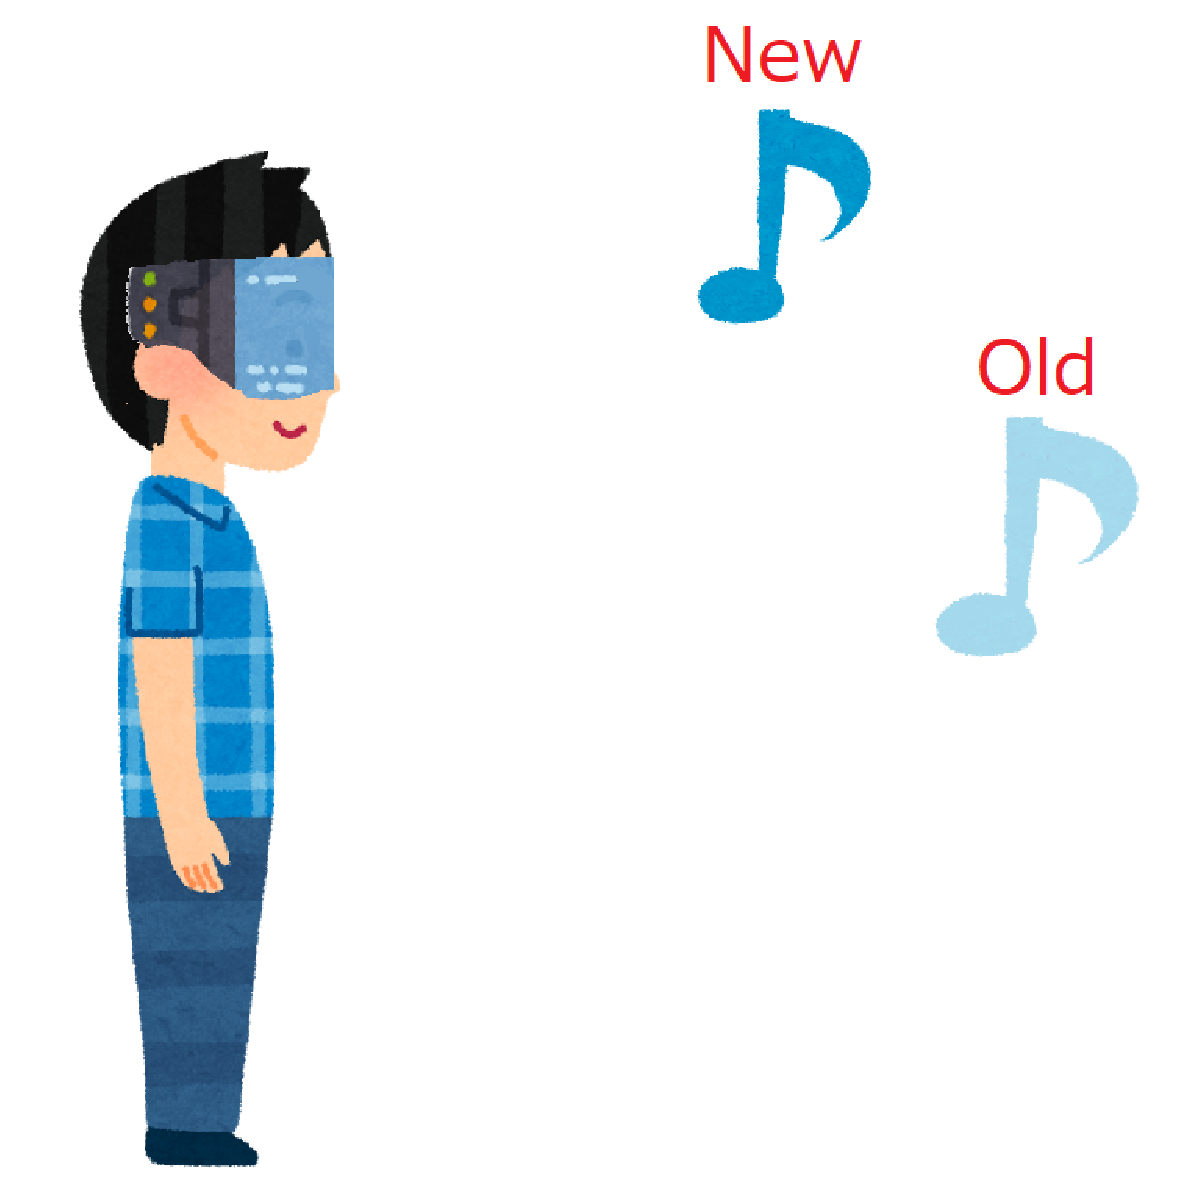
\includegraphics[clip,height=5.0cm,width=6.0cm]{./onpu_memo.eps}
    \caption{3D音符の透明度を変化}
    \ecaption{Change transparency of 3D notes.}
    \label{fig:onpu_memo}
  \end{center}
\end{figure}

\subsubsection{音声によるメモ}
ユーザが思い浮かんだふとしたアイデアは短い言葉だけで表すことが難しい場合もある。そこで、音声によるメモを残す手法を提案する。任意の3D空間上でタップをすることで音声の録音を開始し、もう一度タップすること録音を終了する。その場には3D音符として残る。音声によるメモを聞く際には、3D音符をタップすることで再生することができるようにする。また、音声によるメモが新しいかどうかを一目でわかるように、3D音符の透明度を変化させて表示する手法を提案する(図\ref{fig:onpu_memo})。具体的には古いメモはより透明になるように3D音符を表示する。



\subsection{メモを操作}
広い空間上にメモを残す場合、近くにあるメモだけでなく、遠くにあるメモを移動させることも必要となる。そこで、遠くにあるメモを視線で選択をし、タップアンドホールドを維持した状態で移動させるインタラクションを提案する。また、視線上に複数のメモがある場合、その中の一つをどうやって選択するかという問題が発生することが考えられる。そこで、音声入力によってメモの選択の変更を行う手法を提案する(図\ref{fig:sentaku_memo})。

\begin{figure}[h]
  \begin{center}
    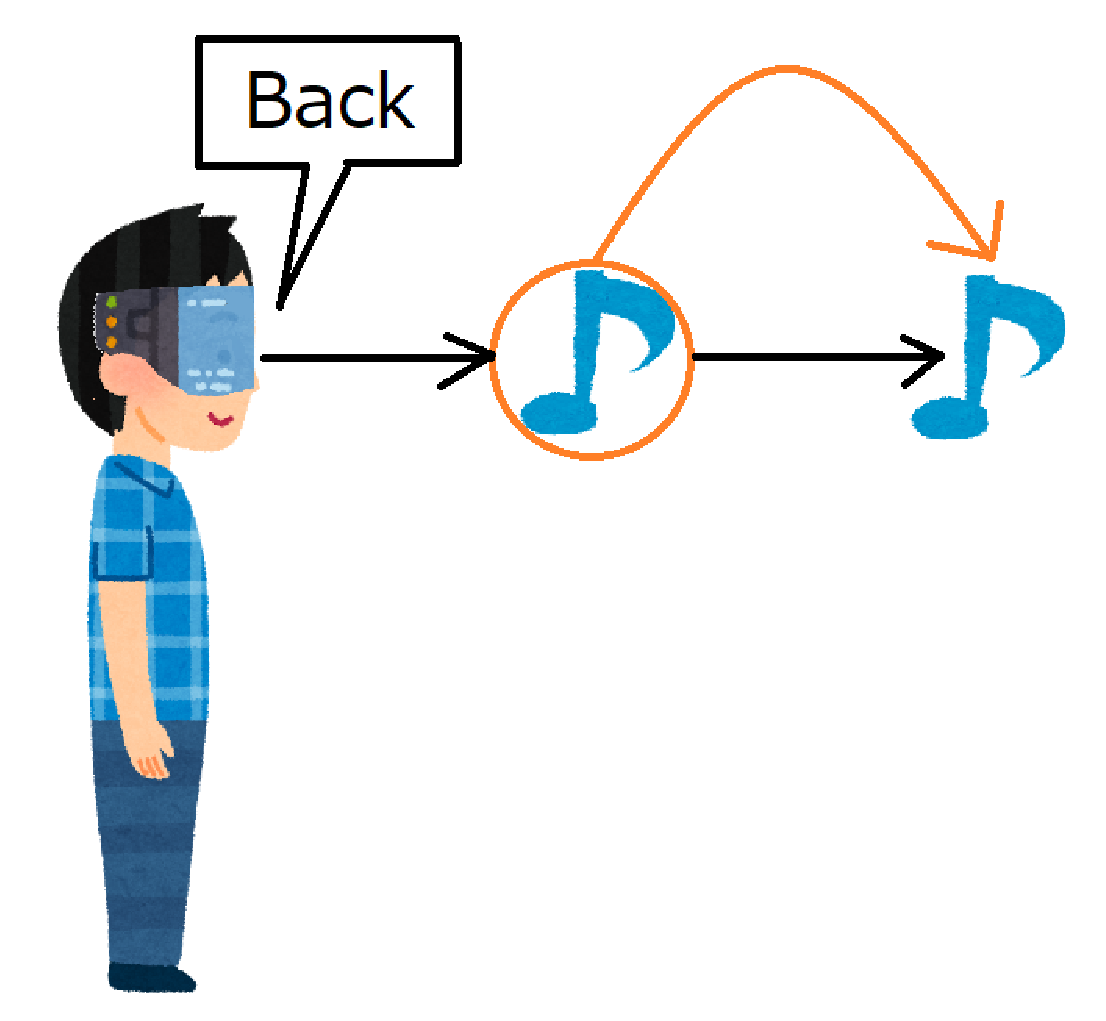
\includegraphics[clip,height=5.0cm,width=6.0cm]{./sentaku_memo.eps}
    \caption{視線上にある複数のメモの中の一つを選択}
    \ecaption{Select one of multiple notes on line of sight.}
    \label{fig:sentaku_memo}
  \end{center}
\end{figure}

\begin{figure*}[t]
  \begin{center}
    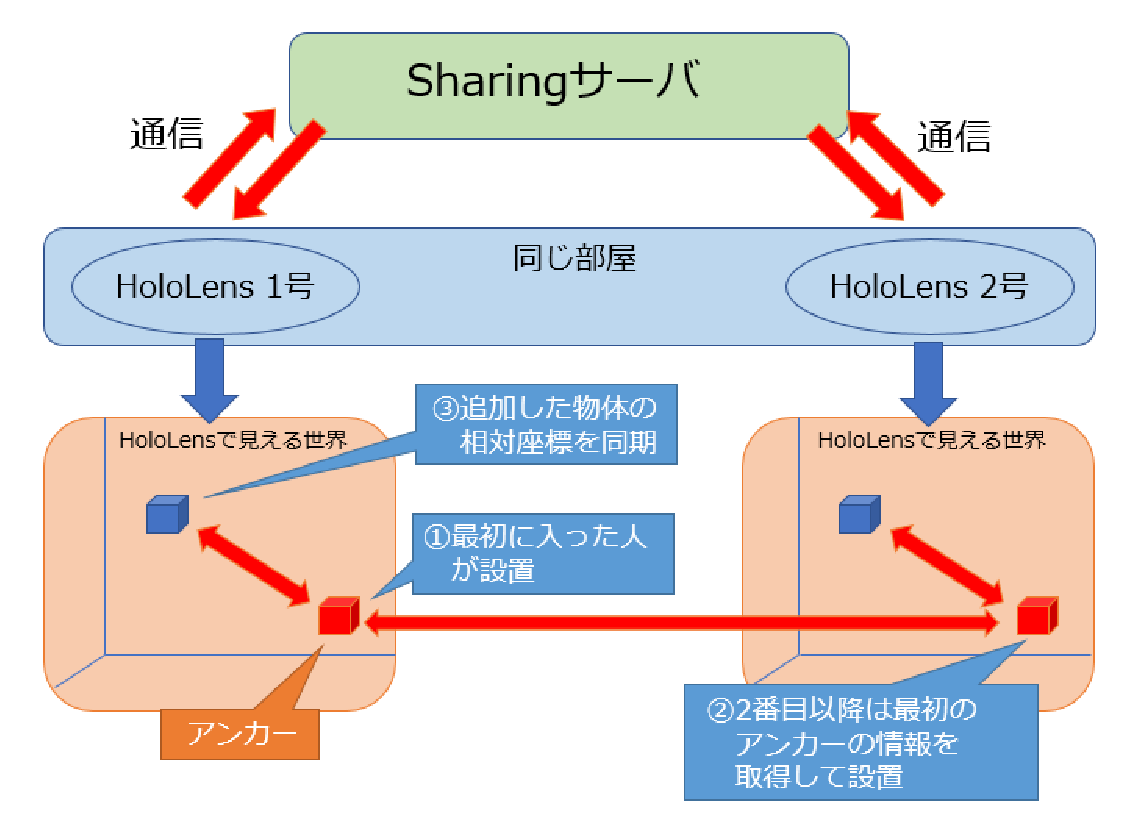
\includegraphics[clip,height=10.0cm,width=14.0cm]{./sharing.eps}
    \caption{アンカーを設置して座標の位置合わせを行い共有}
    \ecaption{Set up an anchor, align coordinates and share.}
    \label{fig:sharing}
  \end{center}
\end{figure*}

\subsection{メモを共有}
実世界の任意の3D空間上に残したメモを他人に見せるには、HoloToolkit\cite{tex7}のSharing\cite{tex8}という機能を利用し、Sharing用のサーバを介して空間の共有を行う。HoloToolkitとはHoloLens向けのアプリを効率的に開発するための機能を含んだツールキットのことである。また、HoloLensで3Dアプリを起動した場合、アプリ内の空間について起動時点のHoloLensの座標と向いている方向を起点として座標軸(0,0,0)、カメラ角(0,0,0)で処理される。このため、同じアプリを他の人が起動するときは寸分違わず同じ場所、同じ向きでアプリを起動しない限り、現実の空間の同じ位置で物体を共有することができないという問題が発生する。この問題を解決するためにはアンカーの共有を行う(図\ref{fig:sharing})。アンカーとは船の錨の意味で空間内で絶対的な位置に居座ることができるオブジェクトのことである。これを設置することで位置合わせを行い、実世界の任意の3D空間上に残したメモの共有を行う。

%%%%%%%%%%%%%%%%%%%%%%%%%%%%%%%%%%%%%%%%%%%%%%%%%%%%%%%%%%%%%%%%%%%%%
\section{システムの試作}
%%%%%%%%%%%%%%%%%%%%%%%%%%%%%%%%%%%%%%%%%%%%%%%%%%%%%%%%%%%%%%%%%%%%%
本システムを作成する前に、実際に動作するかどうか確認を行うために3D描画システムの試作を行った。

\subsection{実装環境}
ハードウェアはHoloLensを利用し、開発環境はWindows10でUnity\cite{tex9}を使用した。Unityとはユニティ・テクノロジーズ社が提供するゲーム開発プラットフォームであり、3D・2D描画やサウンド再生等を備えた統合開発環境である。また、Unity用のHoloLens向けのツールキットであるHoloToolkit-Unityの導入を行った。

\subsection{実装手順}
Unityを起動し、まずメッシュが手に追従するものを作成した。ここでは3D ObjectとしてCubeを追加した。次にSpatialMappingとInputManagerを追加し、カメラをデフォルトのものからHoloLendsCameraに変更した。HoloLensはSpatialMappingと呼ばれる周辺の凹凸を判別する機能を持っており、これによって現実空間にあたり判定をつけ、落下してくる仮想のオブジェクトを現実空間に配置できる。また、Unityで開発する際、この凹凸の情報はメッシュデータとして保持している。InputManagerはキー等の入力の認識を行うが、ここではジェスチャの認識を行った。次に手の検出や位置を受け取るスクリプトを作成し、手の検出と手の状態を保持できるようにし、手の位置を取得をできるようにした。加えて、手の位置にオブジェクトを追従させるようにした。Trail Renderer\cite{tex10}というオブジェクトが動く際に、オブジェクトの後ろに軌跡を作るスクリプトを使用し、3D空間上に複数の線を軌跡を描画できるようにした。最後にそのままの状態だと3D空間上にオブジェクトであるCubeが残ってしまうので、Cubeを透明にする処理を行った。

\subsection{動作確認}
3D描画システムの試作を行い、HoloLens上でシステムを動かして、動作を確認した。図\ref{fig:linedraw}のように3D空間上でタップアンドホールドをした状態を維持している間は、線が表示されるようにし、ホールドを解除すると表示をやめるようにした。3D空間上で手前から奥に線を引くことができることも確認できた。線が表示される位置がタップアンドホールドした位置より少し離れた場所に表示されているので、今後調整する必要があると考えられる。また、図\ref{fig:rittai}のように3D空間上に立体の図形を描き、表示できることも確認できた。

\begin{figure}[h]
  \begin{center}
    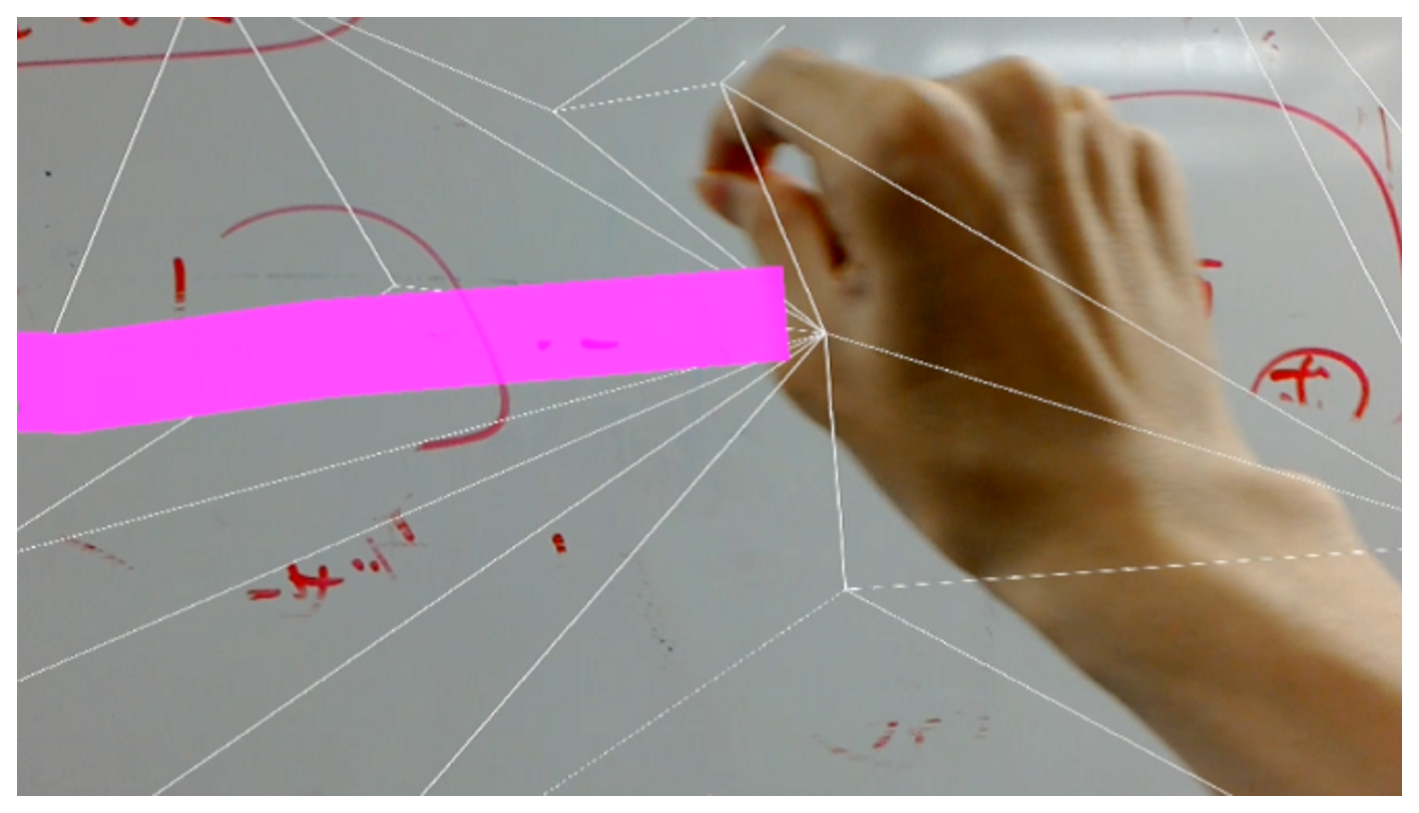
\includegraphics[clip,height=5.0cm,width=7.0cm]{./linedraw.eps}
    \caption{3D空間上に線を描画}
    \ecaption{Line drawn in 3D.}
    \label{fig:linedraw}
  \end{center}
\end{figure}

\begin{figure}[h]
  \begin{center}
    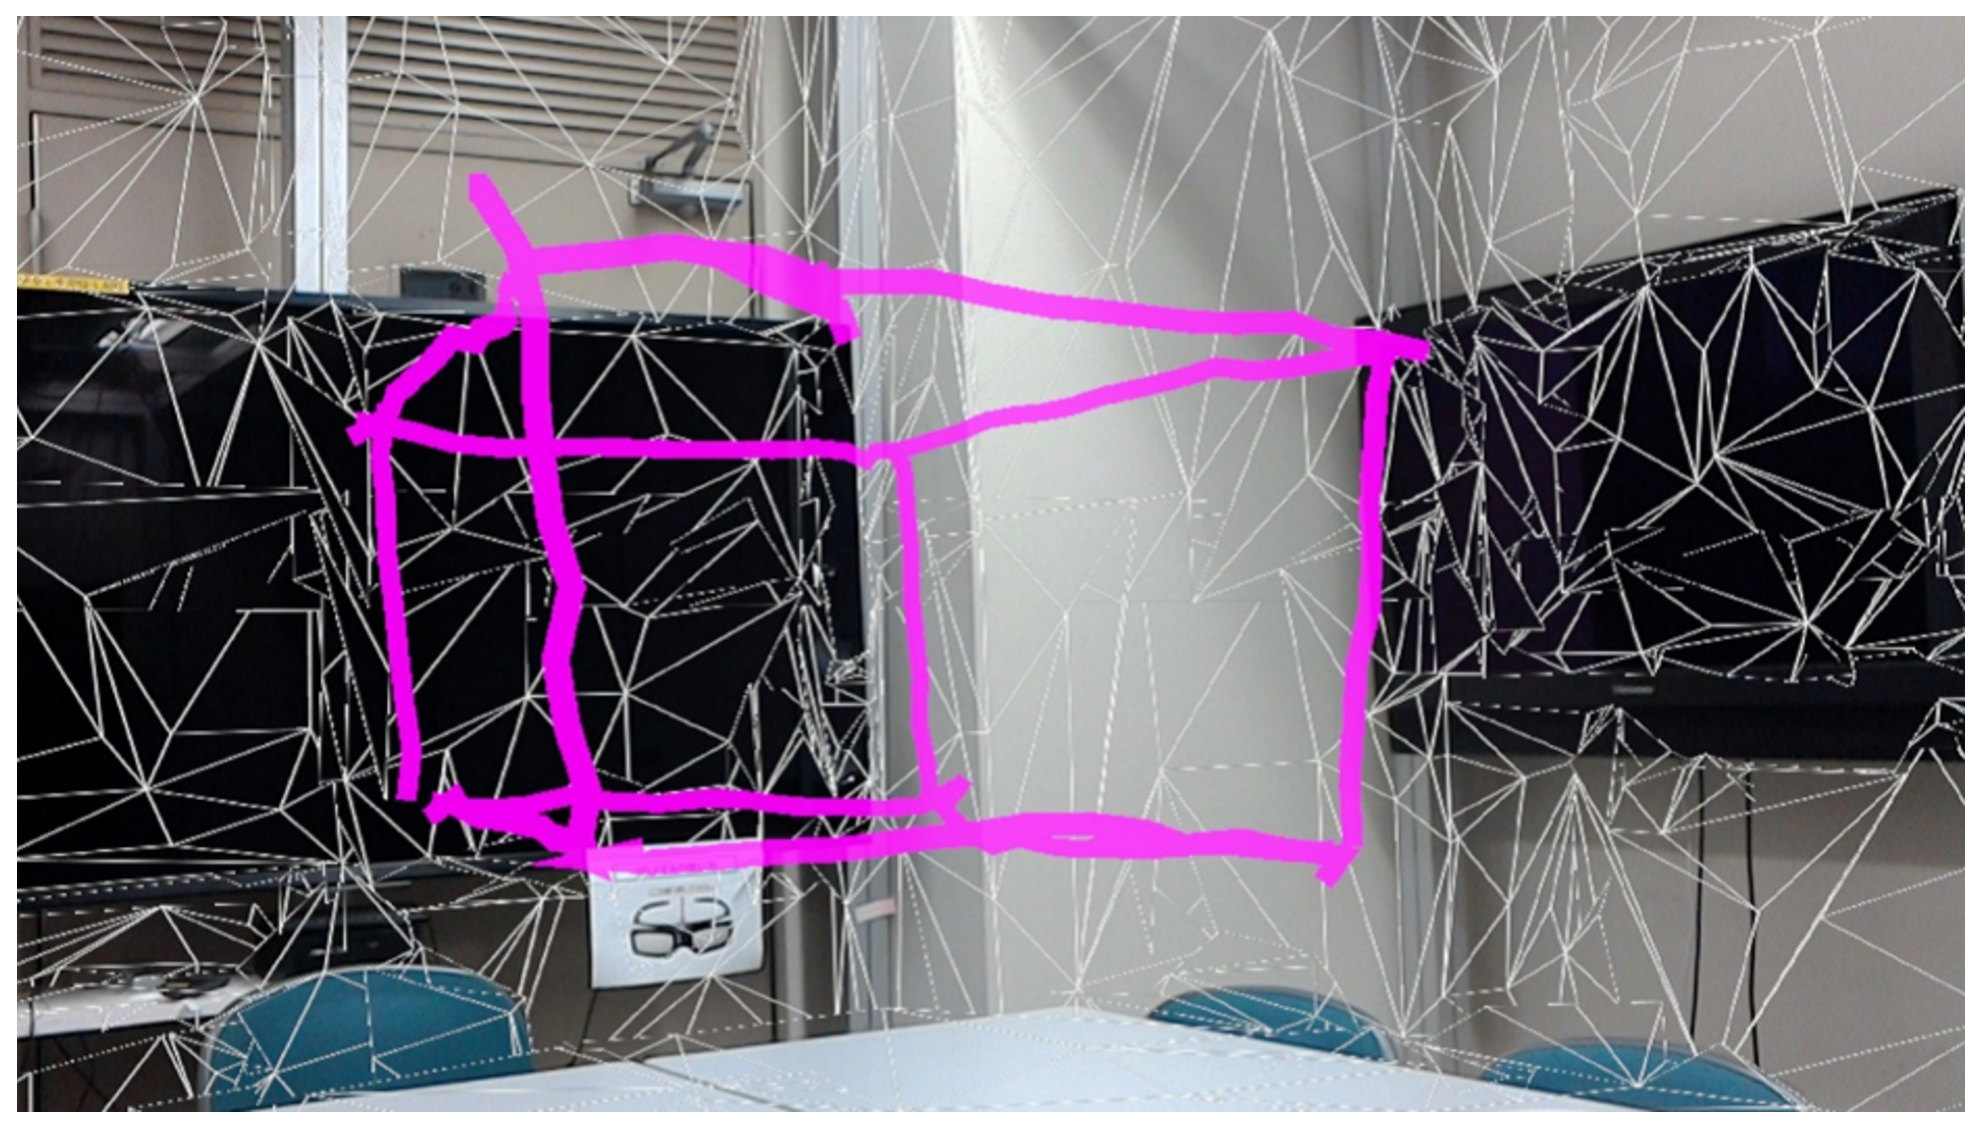
\includegraphics[clip,height=5.0cm,width=7.0cm]{./rittai.eps}
    \caption{3D空間上に立体の図形を描画}
    \ecaption{Three-dimensional figure drawn in 3D.}
    \label{fig:rittai}
  \end{center}
\end{figure}

%%%%%%%%%%%%%%%%%%%%%%%%%%%%%%%%%%%%%%%%%%%%%%%%%%%%%%%%%%%%%%%%%%%%%
\section{おわりに}
%%%%%%%%%%%%%%%%%%%%%%%%%%%%%%%%%%%%%%%%%%%%%%%%%%%%%%%%%%%%%%%%%%%%%
3D空間上の任意の場所にメモを置くことができ、複数人で使用できる3Dアイデアノートシステムの提案を行った。本システムは図形や文字だけでなく、音声によるメモを残すことも可能にする。

また、本システムを作成する前に動作を確認するためにシステムの試作を行った。試作したシステムをHoloLens上で動かし、3D空間上に線を描いたり、立体の図形を描くことができることを確認した。

今後は試作した3D描画システムを調整し、その他の機能についても実装を行っていく。また、メモを共有する機能で、アンカーを設置して位置合わせを行う際に、アンカーと追加した物体の距離がどの程度大きくても同期できるか予備実験を行う必要があると考えられる。その後、本システムの実装をして、本実験を行い、評価を行っていく予定である。


%%%%%%%%%%%%%%%%%%%%%%%%%%%%%%%%%%%%%%%%%%%%%%%%%%%%%%%%%%%%%%%%%%%%%
%  参考文献
%%%%%%%%%%%%%%%%%%%%%%%%%%%%%%%%%%%%%%%%%%%%%%%%%%%%%%%%%%%%%%%%%%%%%
\begin{thebibliography}{99}
\bibitem{tex1}
        山本, 椎尾:
        空気ペン―空間への描画による情報共有-;
        情報処理学会全国大会講演論文集,
        {\bf Vol.59}, No.4, pp.39-40(1999)
\bibitem{tex2}
	椎尾, 山本:
	コミュニケーションツールのための簡易型ARシステム;
	コンピュータソフトウェア, 
        {\bf Vol.19}, No.4, pp.246-253(2002).
\bibitem{tex3}
	高山, 瑞慶山, 田野, 岩田, 橋山:
	実世界コンテキスト・情報を用いたユビキタスインフォーマルコミュニケーションの実装と評価;
	ヒューマンインタフェースシンポジウム2005,
        pp.955-958(2005).
\bibitem{tex4}
        Tano, S., Takayama, T., Iwata, M. and Hashiyama, T.:
        Wearable Computer for Ubiquitous Informal Communication;
        Sixth International Workshop on Smart Appliances and Wearable Computing-IWSAWC 2006-(at 26th IEEE International Conference on Distributed Computing Systems ICDCS),
        pp.1-8(2006).
\bibitem{tex5}
        長田, 佐々木, 島田, 佐藤:
        スマートグラスを用いた仮想空間への手書き情報共有システム;
        情報処理学会第77回全国大会論文集,
        3-205, 206(2015)
\bibitem{tex6}
        Microsoft Inc:
        HoloLens;
        \url{https://www.microsoft.com/ja-jp/hololens}
\bibitem{tex7}
        Microsoft Inc:
        HoloToolkit;
        \url{https://github.com/Microsoft/HoloToolkit-Unity}
\bibitem{tex8}
        HoloToolkit-UnityのSharingの仕組みをできるだけ簡単に理解する; 
        \url{http://qiita.com/miyaura/items/da1d7bd253c3299327ba}
\bibitem{tex9}
        Unity Technologies Inc:
        Unity;
        \url{https://unity3d.com/jp/unity}
\bibitem{tex10}
        TrailRenderer;
        \url{https://docs.unity3d.com/ja/540/ScriptReference/TrailRenderer.html}

\end{thebibliography}


\end{document}

